\chapter{Partilhas de ficheiros}
\label{cap5}

\section{Enquadramento do cap\'{\i}tulo}

Este cap\'{\i}tulo apresenta a implementa\c{c}\~ao dos pontos do enunciado relacionados com partilhas de ficheiros em ambiente cliente-servidor. O foco recai sobre dois servi\c{c}os complementares: partilhas para clientes Windows atrav\'es de Samba (P2) e partilhas para clientes Linux/Unix atrav\'es de NFS (P7).

Em termos funcionais, o Samba permite disponibilizar diret\'orios Linux usando protocolos compat\'iveis com o ecossistema Windows, enquanto o NFS fornece um mecanismo nativo e leve de partilha para sistemas Unix-like. A combina\c{c}\~ao dos dois servi\c{c}os permite cobrir cen\'arios heterog\'eneos de acesso a ficheiros no mesmo laborat\'orio.

\section{Quest\~ao 2: partilhas com SAMBA}
\label{sec:q2}

\subsection{Objetivo}

A Quest\~ao 2 teve como objetivo automatizar a configura\c{c}\~ao do servi\c{c}o Samba no servidor Linux, permitindo a cria\c{c}\~ao de partilhas do sistema de ficheiros acess\'iveis a m\'aquinas Windows. Para al\'em da cria\c{c}\~ao inicial de partilhas, a aplica\c{c}\~ao desenvolvida passou tamb\'em a suportar opera\c{c}\~oes de administra\c{c}\~ao corrente, nomeadamente elimina\c{c}\~ao, altera\c{c}\~ao e desativa\c{c}\~ao de partilhas j\'a existentes.

O enunciado exigia ainda a possibilidade de mapear no servidor Linux partilhas realizadas em m\'aquinas Windows. Por esse motivo, a solu\c{c}\~ao implementada incluiu n\~ao apenas a gest\~ao do ficheiro de configura\c{c}\~ao do Samba, mas tamb\'em a capacidade de montar partilhas SMB/CIFS remotas no pr\'oprio sistema Linux.

Desta forma, a aplica\c{c}\~ao deixou de atuar apenas como mecanismo de publica\c{c}\~ao de partilhas para clientes Windows, passando tamb\'em a suportar o acesso inverso do Linux a recursos partilhados por sistemas Windows.

\subsection{Implementa\c{c}\~ao}

O script \texttt{q2\_samba.sh} foi desenvolvido para concentrar num \'unico ponto as principais opera\c{c}\~oes de administra\c{c}\~ao do servi\c{c}o Samba. A sua estrutura assenta num menu interativo que permite ao utilizador criar, eliminar, alterar e desativar partilhas no ficheiro \texttt{/etc/samba/smb.conf}, bem como montar partilhas Windows no servidor Linux.

Numa primeira fase, o script define o caminho do ficheiro principal de configura\c{c}\~ao do Samba e a diretoria base a partir da qual podem ser criadas partilhas locais.

\textbf{Listagem 1}

Estrutura base do script

\begin{lstlisting}[language=bash,breaklines=true,basicstyle=\ttfamily\small,columns=fullflexible,keepspaces=true,showstringspaces=false]
SMB_CONF="/etc/samba/smb.conf"
BASE_DIR="/partilhas"
\end{lstlisting}

Estas vari\'aveis delimitam a \'area de atua\c{c}\~ao do script. O ficheiro \texttt{smb.conf} constitui o centro da configura\c{c}\~ao do servi\c{c}o Samba, sendo nele que s\~ao declaradas as diferentes partilhas disponibilizadas pelo servidor. J\'a a diretoria base \texttt{/partilhas} funciona como localiza\c{c}\~ao padr\~ao para cria\c{c}\~ao autom\'atica das pastas exportadas, contribuindo para uma organiza\c{c}\~ao uniforme.

Antes de qualquer opera\c{c}\~ao, o script verifica se o Samba est\'a corretamente dispon\'ivel no sistema.

\textbf{Listagem 2}

Verifica\c{c}\~ao da exist\^encia da configura\c{c}\~ao Samba

\begin{lstlisting}[language=bash,breaklines=true,basicstyle=\ttfamily\small,columns=fullflexible,keepspaces=true,showstringspaces=false]
verifica_samba() {
    if [ ! -f "$SMB_CONF" ]; then
        echo "Erro: $SMB_CONF nao existe."
        echo "Instale primeiro o Samba: yum install samba samba-client -y"
        exit 1
    fi
}
\end{lstlisting}

Este bloco assegura que o ficheiro de configura\c{c}\~ao principal do Samba existe efetivamente no sistema. A sua import\^ancia reside em evitar que o script tente manipular uma configura\c{c}\~ao inexistente.

Sempre que o \texttt{smb.conf} \'e alterado, o script valida a sua consist\^encia antes de reiniciar o servi\c{c}o.

\textbf{Listagem 3}

Valida\c{c}\~ao da configura\c{c}\~ao e rein\'icio do servi\c{c}o

\begin{lstlisting}[language=bash,breaklines=true,basicstyle=\ttfamily\small,columns=fullflexible,keepspaces=true,showstringspaces=false]
reinicia_samba() {
    testparm -s >/dev/null 2>&1
    if [ $? -ne 0 ]; then
        echo "Erro na configuracao do Samba. Verifique o smb.conf."
        exit 1
    fi

    systemctl enable smb --now
    systemctl restart smb
    echo "Servico smb reiniciado com sucesso."
}
\end{lstlisting}

O comando \texttt{testparm} verifica a validade sint\'atica do ficheiro \texttt{smb.conf}, permitindo detetar erros antes da aplica\c{c}\~ao efetiva da configura\c{c}\~ao. S\'o depois dessa valida\c{c}\~ao \'e que o servi\c{c}o \texttt{smb} \'e ativado e reiniciado.

A primeira funcionalidade principal do script corresponde \`a cria\c{c}\~ao de partilhas Samba.

\textbf{Listagem 4}

Cria\c{c}\~ao de partilhas Samba

\begin{lstlisting}[language=bash,breaklines=true,basicstyle=\ttfamily\small,columns=fullflexible,keepspaces=true,showstringspaces=false]
criar_partilha() {
    read -p "Nome da partilha: " NOME
    read -p "Diretoria da partilha [/partilhas/$NOME]: " CAMINHO

    [ -z "$CAMINHO" ] && CAMINHO="$BASE_DIR/$NOME"

    if grep -q "^\[$NOME\]" "$SMB_CONF"; then
        echo "Erro: a partilha ja existe."
        return
    fi

    mkdir -p "$CAMINHO"
    chmod 777 "$CAMINHO"

    cat >> "$SMB_CONF" <<EOF

[$NOME]
    path = $CAMINHO
    browseable = yes
    writable = yes
    guest ok = yes
    read only = no
EOF

    echo "Partilha criada."
    reinicia_samba
}
\end{lstlisting}

Este bloco automatiza tr\^es tarefas que normalmente seriam manuais: cria\c{c}\~ao da diretoria f\'isica, defini\c{c}\~ao de permiss\~oes e inser\c{c}\~ao da sec\c{c}\~ao no \texttt{smb.conf}. O script previne ainda duplica\c{c}\~oes, verificando se j\'a existe uma partilha com o mesmo nome.

A segunda opera\c{c}\~ao principal \'e a elimina\c{c}\~ao de partilhas.

\textbf{Listagem 5}

Elimina\c{c}\~ao de partilhas Samba

\begin{lstlisting}[language=bash,breaklines=true,basicstyle=\ttfamily\small,columns=fullflexible,keepspaces=true,showstringspaces=false]
eliminar_partilha() {
    read -p "Nome da partilha a eliminar: " NOME

    if ! grep -Eq "^#?\[$NOME\]" "$SMB_CONF"; then
        echo "Erro: partilha nao encontrada."
        return
    fi

    awk -v share="$NOME" '
    BEGIN {skip=0}
    $0 ~ "^#?\\["share"\\]$" {skip=1; next}
    $0 ~ "^#?\\[.*\\]$" && skip==1 {skip=0}
    skip==0 {print}
    ' "$SMB_CONF" > /tmp/smb.conf.new && mv /tmp/smb.conf.new "$SMB_CONF"

    echo "Partilha eliminada do smb.conf."
    reinicia_samba
}
\end{lstlisting}

Em vez de remover apenas uma linha, o script elimina todo o bloco da partilha no ficheiro de configura\c{c}\~ao. Esta op\c{c}\~ao \'e a mais adequada porque cada partilha no Samba \'e definida por v\'arias diretivas.

O script inclui tamb\'em a possibilidade de alterar par\^ametros de uma partilha j\'a existente.

\textbf{Listagem 6}

Altera\c{c}\~ao de partilhas existentes

\begin{lstlisting}[language=bash,breaklines=true,basicstyle=\ttfamily\small,columns=fullflexible,keepspaces=true,showstringspaces=false]
alterar_partilha() {
    read -p "Nome da partilha a alterar: " NOME
    ...
    sed -i "/^\[$NOME\]/,/^\[/ s|^[[:space:]]*path = .*|    path = $NOVO_PATH|" "$SMB_CONF"
    ...
}
\end{lstlisting}

Esta funcionalidade acrescenta flexibilidade administrativa. O utilizador pode alterar caminho, estado de escrita, acesso an\'onimo e pol\'itica de leitura sem reescrever a partilha do zero. A utiliza\c{c}\~ao de \texttt{sed} limitada ao intervalo da partilha evita altera\c{c}\~oes noutras sec\c{c}\~oes.

Outra opera\c{c}\~ao prevista \'e a desativa\c{c}\~ao de partilhas.

\textbf{Listagem 7}

Desativa\c{c}\~ao de partilhas

\begin{lstlisting}[language=bash,breaklines=true,basicstyle=\ttfamily\small,columns=fullflexible,keepspaces=true,showstringspaces=false]
desativar_partilha() {
    read -p "Nome da partilha a desativar: " NOME
    ...
    sed -i "/^\[$NOME\]/,/^\[/ s/^/#/" "$SMB_CONF"
    ...
}
\end{lstlisting}

Aqui foi adotada uma estrat\'egia n\~ao destrutiva: em vez de apagar, o bloco \'e comentado. Isto permite suspender a partilha sem perder a configura\c{c}\~ao.

Por fim, o script integra a capacidade de montar partilhas Windows no Linux.

\textbf{Listagem 8}

Montagem de partilhas Windows no servidor Linux

\begin{lstlisting}[language=bash,breaklines=true,basicstyle=\ttfamily\small,columns=fullflexible,keepspaces=true,showstringspaces=false]
montar_partilha_windows() {
    if ! command -v mount.cifs >/dev/null 2>&1; then
        yum install cifs-utils -y || return
    fi

    read -p "IP ou nome da maquina Windows: " HOST
    read -p "Nome da partilha Windows: " SHARE
    read -p "Ponto de montagem local: " MNT
    read -p "Utilizador Windows: " USER

    mkdir -p "$MNT"
    mount -t cifs "//$HOST/$SHARE" "$MNT" -o username="$USER"
}
\end{lstlisting}

Este bloco responde diretamente ao requisito de mapear no Linux partilhas SMB/CIFS disponibilizadas por m\'aquinas Windows.

Todas as opera\c{c}\~oes foram reunidas num menu \'unico.

\textbf{Listagem 9}

Menu de gest\~ao do Samba

\begin{lstlisting}[language=bash,breaklines=true,basicstyle=\ttfamily\small,columns=fullflexible,keepspaces=true,showstringspaces=false]
menu() {
    echo "===== MENU SAMBA ====="
    echo "1 - Criar partilha"
    echo "2 - Eliminar partilha"
    echo "3 - Alterar partilha"
    echo "4 - Desativar partilha"
    echo "5 - Montar partilha Windows no Linux"
    echo "0 - Sair"
}
\end{lstlisting}

A exist\^encia deste menu melhora a usabilidade e torna o script mais pr\'oximo de uma ferramenta de administra\c{c}\~ao para opera\c{c}\~oes correntes de Samba.

\subsection{Valida\c{c}\~ao funcional}

A valida\c{c}\~ao da Quest\~ao 2 foi realizada atrav\'es da execu\c{c}\~ao do script no servidor e da verifica\c{c}\~ao pr\'atica das opera\c{c}\~oes de cria\c{c}\~ao, altera\c{c}\~ao, desativa\c{c}\~ao e elimina\c{c}\~ao de partilhas, bem como da montagem de partilhas Windows no sistema Linux.

Numa primeira fase, o script foi executado com permiss\~oes de administra\c{c}\~ao e foi criada uma nova partilha (\texttt{24845}). Em seguida, confirmou-se no \texttt{smb.conf} a cria\c{c}\~ao da sec\c{c}\~ao correspondente, com os par\^ametros esperados (\texttt{path}, \texttt{browseable}, \texttt{writable}, \texttt{guest ok}, \texttt{read only}).

Numa segunda fase, foram testadas as funcionalidades de desativa\c{c}\~ao e elimina\c{c}\~ao. A desativa\c{c}\~ao comentou o bloco da partilha no \texttt{smb.conf}, mantendo a configura\c{c}\~ao para eventual reativa\c{c}\~ao. A elimina\c{c}\~ao removeu o bloco da configura\c{c}\~ao de forma definitiva.

Numa terceira fase, testou-se a altera\c{c}\~ao da partilha, atualizando o caminho para \texttt{/partilhas/24845}. A verifica\c{c}\~ao posterior no ficheiro confirmou a altera\c{c}\~ao aplicada.

Por fim, validou-se a montagem de uma partilha Windows no Linux, usando a op\c{c}\~ao 5 do menu. A montagem foi efetuada em \texttt{/mnt/teste} e confirmada com \texttt{mount | grep cifs}. A cria\c{c}\~ao/leitura de ficheiros nesse ponto de montagem comprovou o acesso funcional \`a partilha remota.

Em todas as altera\c{c}\~oes locais de configura\c{c}\~ao, o script executou \texttt{testparm} antes do rein\'icio do servi\c{c}o \texttt{smb}, garantindo consist\^encia sint\'atica do \texttt{smb.conf}.

\subsection{Evid\^encias visuais da Quest\~ao 2}

As evid\^encias seguintes demonstram a execu\c{c}\~ao das opera\c{c}\~oes principais do script e a valida\c{c}\~ao da montagem CIFS no servidor Linux.

\begin{figure}[!htbp]
\centering
\IfFileExists{figuras/q2_menu_criar.png}{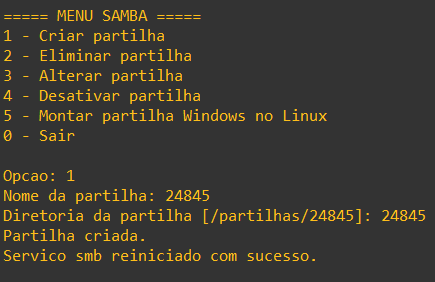
\includegraphics[width=0.78\textwidth,height=0.72\textheight,keepaspectratio]{figuras/q2_menu_criar.png}}{\fbox{\parbox{0.7\textwidth}{Imagem em falta: \texttt{figuras/q2\_menu\_criar.png}}}}
\caption{Menu Samba e cria\c{c}\~ao da partilha 24845}
\end{figure}

\begin{figure}[!htbp]
\centering
\IfFileExists{figuras/q2_smbconf_partilha_criada.png}{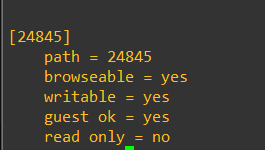
\includegraphics[width=0.78\textwidth,height=0.72\textheight,keepaspectratio]{figuras/q2_smbconf_partilha_criada.png}}{\fbox{\parbox{0.7\textwidth}{Imagem em falta: \texttt{figuras/q2\_smbconf\_partilha\_criada.png}}}}
\caption{Bloco da partilha no \texttt{smb.conf} ap\'os cria\c{c}\~ao}
\end{figure}

\begin{figure}[!htbp]
\centering
\IfFileExists{figuras/q2_menu_desativar.png}{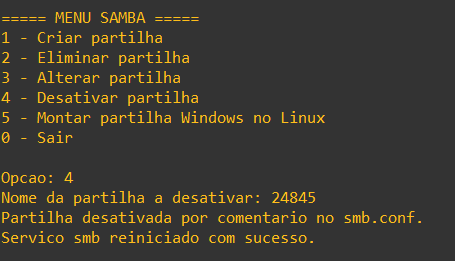
\includegraphics[width=0.78\textwidth,height=0.72\textheight,keepaspectratio]{figuras/q2_menu_desativar.png}}{\fbox{\parbox{0.7\textwidth}{Imagem em falta: \texttt{figuras/q2\_menu\_desativar.png}}}}
\caption{Desativa\c{c}\~ao de partilha pelo menu}
\end{figure}

\begin{figure}[!htbp]
\centering
\IfFileExists{figuras/q2_smbconf_partilha_comentada.png}{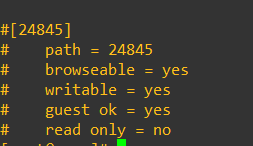
\includegraphics[width=0.78\textwidth,height=0.72\textheight,keepaspectratio]{figuras/q2_smbconf_partilha_comentada.png}}{\fbox{\parbox{0.7\textwidth}{Imagem em falta: \texttt{figuras/q2\_smbconf\_partilha\_comentada.png}}}}
\caption{Partilha comentada no \texttt{smb.conf} ap\'os desativa\c{c}\~ao}
\end{figure}

\begin{figure}[!htbp]
\centering
\IfFileExists{figuras/q2_menu_eliminar.png}{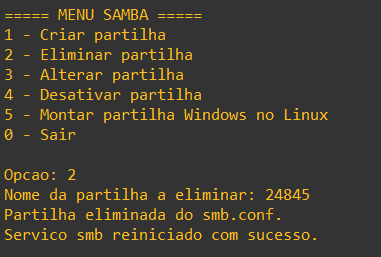
\includegraphics[width=0.78\textwidth,height=0.72\textheight,keepaspectratio]{figuras/q2_menu_eliminar.png}}{\fbox{\parbox{0.7\textwidth}{Imagem em falta: \texttt{figuras/q2\_menu\_eliminar.png}}}}
\caption{Elimina\c{c}\~ao da partilha pelo menu}
\end{figure}

\begin{figure}[!htbp]
\centering
\IfFileExists{figuras/q2_smbconf_global.png}{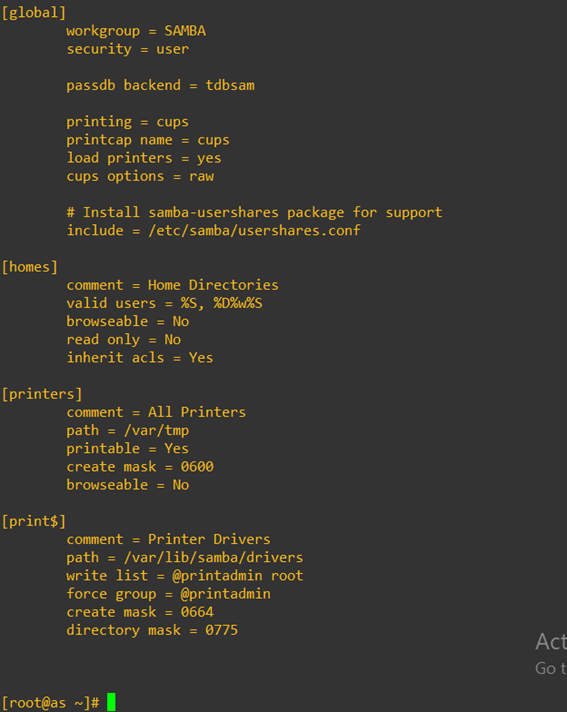
\includegraphics[width=0.78\textwidth,height=0.72\textheight,keepaspectratio]{figuras/q2_smbconf_global.png}}{\fbox{\parbox{0.7\textwidth}{Imagem em falta: \texttt{figuras/q2\_smbconf\_global.png}}}}
\caption{Excerto da configura\c{c}\~ao global do Samba}
\end{figure}

\begin{figure}[!htbp]
\centering
\IfFileExists{figuras/q2_menu_alterar.png}{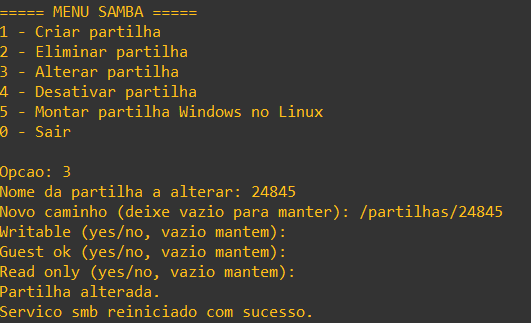
\includegraphics[width=0.78\textwidth,height=0.72\textheight,keepaspectratio]{figuras/q2_menu_alterar.png}}{\fbox{\parbox{0.7\textwidth}{Imagem em falta: \texttt{figuras/q2\_menu\_alterar.png}}}}
\caption{Altera\c{c}\~ao de par\^ametros da partilha}
\end{figure}

\begin{figure}[!htbp]
\centering
\IfFileExists{figuras/q2_smbconf_partilha_alterada.png}{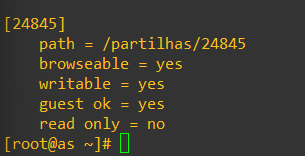
\includegraphics[width=0.78\textwidth,height=0.72\textheight,keepaspectratio]{figuras/q2_smbconf_partilha_alterada.png}}{\fbox{\parbox{0.7\textwidth}{Imagem em falta: \texttt{figuras/q2\_smbconf\_partilha\_alterada.png}}}}
\caption{Partilha ap\'os altera\c{c}\~ao do caminho}
\end{figure}

\begin{figure}[!htbp]
\centering
\IfFileExists{figuras/q2_montagem_menu.png}{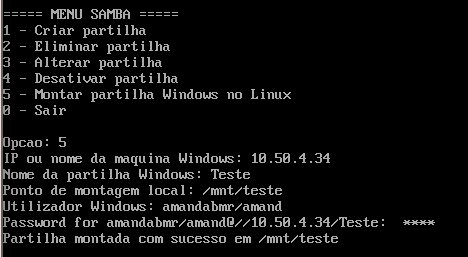
\includegraphics[width=0.78\textwidth,height=0.72\textheight,keepaspectratio]{figuras/q2_montagem_menu.png}}{\fbox{\parbox{0.7\textwidth}{Imagem em falta: \texttt{figuras/q2\_montagem\_menu.png}}}}
\caption{Montagem de partilha Windows no Linux}
\end{figure}

\begin{figure}[!htbp]
\centering
\IfFileExists{figuras/q2_montagem_validacao.png}{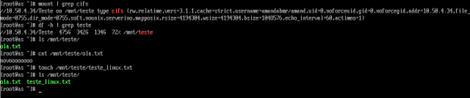
\includegraphics[width=0.78\textwidth,height=0.72\textheight,keepaspectratio]{figuras/q2_montagem_validacao.png}}{\fbox{\parbox{0.7\textwidth}{Imagem em falta: \texttt{figuras/q2\_montagem\_validacao.png}}}}
\caption{Valida\c{c}\~ao da montagem CIFS em \texttt{/mnt/teste}}
\end{figure}

\clearpage
\section{Quest\~ao 7: configura\c{c}\~ao autom\'atica do servi\c{c}o NFS}
\label{sec:q7}

\subsection{Objetivo}

A Quest\~ao 7 teve como objetivo automatizar a configura\c{c}\~ao do servi\c{c}o NFS no servidor Linux, permitindo a cria\c{c}\~ao de partilhas do sistema de ficheiros para m\'aquinas Linux/Unix atrav\'es do ficheiro \texttt{/etc/exports}. Para al\'em da cria\c{c}\~ao inicial das partilhas, a aplica\c{c}\~ao desenvolvida passou tamb\'em a suportar opera\c{c}\~oes de elimina\c{c}\~ao, altera\c{c}\~ao e desativa\c{c}\~ao de exporta\c{c}\~oes j\'a existentes.

O enunciado exigia ainda a valida\c{c}\~ao pr\'atica do mapeamento NFS numa m\'aquina cliente Linux, utilizando o comando \texttt{mount -t nfs}. Por esse motivo, a solu\c{c}\~ao implementada n\~ao se limitou \`a altera\c{c}\~ao do ficheiro \texttt{/etc/exports}, incluindo tamb\'em a aplica\c{c}\~ao imediata das exporta\c{c}\~oes e a verifica\c{c}\~ao do seu funcionamento efetivo no cliente.

Desta forma, o projeto passou a abranger n\~ao apenas a configura\c{c}\~ao local do servi\c{c}o NFS, mas tamb\'em a confirma\c{c}\~ao da sua utiliza\c{c}\~ao real em ambiente cliente-servidor.

\subsection{Implementa\c{c}\~ao}

O script \texttt{q7\_nfs.sh} foi desenvolvido para centralizar num \'unico ponto as principais opera\c{c}\~oes de administra\c{c}\~ao do servi\c{c}o NFS. A sua l\'ogica organiza-se em torno de um menu interativo que permite criar, eliminar, alterar e desativar partilhas, bem como listar as exporta\c{c}\~oes ativas do servidor.

Numa primeira fase, o script define o caminho do ficheiro principal de exporta\c{c}\~oes e a diretoria base a utilizar na cria\c{c}\~ao autom\'atica das partilhas.

\textbf{Listagem 36}

Estrutura base do script

\begin{lstlisting}[language=bash,breaklines=true,basicstyle=\ttfamily\small,columns=fullflexible,keepspaces=true,showstringspaces=false]
EXPORTS="/etc/exports"
BASE_DIR="/partilhas"
\end{lstlisting}

Estas vari\'aveis delimitam a \'area principal de atua\c{c}\~ao da solu\c{c}\~ao. O ficheiro \texttt{/etc/exports} \'e o elemento central da configura\c{c}\~ao NFS, sendo nele que s\~ao declaradas as diretorias partilhadas, os clientes autorizados e as op\c{c}\~oes de exporta\c{c}\~ao. J\'a a diretoria \texttt{/partilhas} funciona como localiza\c{c}\~ao padr\~ao para a cria\c{c}\~ao autom\'atica das pastas exportadas, contribuindo para uma organiza\c{c}\~ao consistente do sistema de ficheiros.

Antes de qualquer opera\c{c}\~ao, o script verifica se o servi\c{c}o NFS est\'a dispon\'ivel no sistema e garante a exist\^encia do ficheiro de exporta\c{c}\~oes.

\textbf{Listagem 37}

Verifica\c{c}\~ao da disponibilidade do NFS

\begin{lstlisting}[language=bash,breaklines=true,basicstyle=\ttfamily\small,columns=fullflexible,keepspaces=true,showstringspaces=false]
verifica_nfs() {
    if ! command -v exportfs >/dev/null 2>&1; then
        echo "Erro: NFS nao instalado."
        echo "Execute: yum install nfs-utils -y"
        exit 1
    fi

    if [ ! -f "$EXPORTS" ]; then
        touch "$EXPORTS"
    fi
}
\end{lstlisting}

Este bloco impede a execu\c{c}\~ao do script num sistema que n\~ao disponha do servi\c{c}o NFS ou das ferramentas necess\'arias \`a gest\~ao das exporta\c{c}\~oes.

Sempre que o ficheiro de exporta\c{c}\~oes \'e alterado, o script aplica de imediato a nova configura\c{c}\~ao ao sistema.

\textbf{Listagem 38}

Aplica\c{c}\~ao das exporta\c{c}\~oes NFS

\begin{lstlisting}[language=bash,breaklines=true,basicstyle=\ttfamily\small,columns=fullflexible,keepspaces=true,showstringspaces=false]
aplica_exports() {
    exportfs -ra
    if [ $? -ne 0 ]; then
        echo "Erro ao atualizar exportacoes NFS."
        exit 1
    fi

    systemctl enable nfs-server --now
    systemctl restart nfs-server
    echo "Configuracao NFS aplicada com sucesso."
}
\end{lstlisting}

O comando \texttt{exportfs -ra} for\c{c}a a releitura do ficheiro \texttt{/etc/exports} e reaplica as exporta\c{c}\~oes definidas. Esta abordagem garante que qualquer altera\c{c}\~ao introduzida pelo utilizador passa imediatamente a refletir-se no servi\c{c}o ativo.

A primeira funcionalidade principal do script corresponde \`a cria\c{c}\~ao de partilhas NFS.

\textbf{Listagem 39}

Cria\c{c}\~ao de partilhas NFS

\begin{lstlisting}[language=bash,breaklines=true,basicstyle=\ttfamily\small,columns=fullflexible,keepspaces=true,showstringspaces=false]
criar_partilha() {
    read -p "Nome da partilha: " NOME
    read -p "Diretoria da partilha [/partilhas/$NOME]: " CAMINHO
    read -p "Rede/host autorizado (ex: 10.50.2.0/24): " REDE
    read -p "Opcoes NFS [rw,sync,no_root_squash]: " OPCOES

    [ -z "$CAMINHO" ] && CAMINHO="$BASE_DIR/$NOME"
    [ -z "$OPCOES" ] && OPCOES="rw,sync,no_root_squash"

    if grep -q "^$CAMINHO " "$EXPORTS"; then
        echo "Erro: ja existe uma exportacao para $CAMINHO"
        return
    fi

    mkdir -p "$CAMINHO"
    chmod 777 "$CAMINHO"

    echo "$CAMINHO $REDE($OPCOES)" >> "$EXPORTS"

    echo "Partilha NFS criada:"
    echo "$CAMINHO $REDE($OPCOES)"
    aplica_exports
}
\end{lstlisting}

Este bloco automatiza simultaneamente a cria\c{c}\~ao da diretoria f\'isica, a atribui\c{c}\~ao de permiss\~oes e a escrita da linha correspondente no ficheiro \texttt{/etc/exports}, prevenindo ainda duplica\c{c}\~oes de exporta\c{c}\~oes.

A segunda opera\c{c}\~ao principal corresponde \`a elimina\c{c}\~ao de partilhas existentes.

\textbf{Listagem 40}

Elimina\c{c}\~ao de partilhas NFS

\begin{lstlisting}[language=bash,breaklines=true,basicstyle=\ttfamily\small,columns=fullflexible,keepspaces=true,showstringspaces=false]
eliminar_partilha() {
    read -p "Diretoria da partilha a eliminar: " CAMINHO

    if ! grep -Eq "^#?$CAMINHO " "$EXPORTS"; then
        echo "Erro: partilha nao encontrada."
        return
    fi

    grep -Ev "^#?$CAMINHO " "$EXPORTS" > /tmp/exports.new
    mv /tmp/exports.new "$EXPORTS"

    echo "Partilha removida do /etc/exports."

    exportfs -ra
    if [ $? -ne 0 ]; then
        echo "Erro ao atualizar exportacoes NFS."
        exit 1
    fi

    read -p "Deseja apagar tambem a diretoria $CAMINHO ? (s/n): " OP
    if [ "$OP" = "s" ] || [ "$OP" = "S" ]; then
        rm -rf "$CAMINHO"
        echo "Diretoria removida."
    fi

    systemctl restart nfs-server
    echo "Configuracao NFS aplicada com sucesso."
}
\end{lstlisting}

Este bloco remove do ficheiro \texttt{/etc/exports} a linha correspondente \`a partilha indicada e reaplica a configura\c{c}\~ao. Al\'em disso, permite ao utilizador decidir se pretende remover tamb\'em a diretoria f\'isica associada.

O script suporta tamb\'em a altera\c{c}\~ao de partilhas previamente configuradas.

\textbf{Listagem 41}

Altera\c{c}\~ao de partilhas existentes

\begin{lstlisting}[language=bash,breaklines=true,basicstyle=\ttfamily\small,columns=fullflexible,keepspaces=true,showstringspaces=false]
alterar_partilha() {
    read -p "Diretoria da partilha a alterar: " CAMINHO

    if ! grep -Eq "^#?$CAMINHO " "$EXPORTS"; then
        echo "Erro: partilha nao encontrada."
        return
    fi

    LINHA_ATUAL=$(grep -E "^#?$CAMINHO " "$EXPORTS" | head -n 1)
    echo "Linha atual: $LINHA_ATUAL"

    read -p "Nova rede/host (vazio mantem): " NOVA_REDE
    read -p "Novas opcoes (vazio mantem): " NOVAS_OPCOES

    HOST_ATUAL=$(echo "$LINHA_ATUAL" | awk '{print $2}' | cut -d'(' -f1)
    OPCOES_ATUAIS=$(echo "$LINHA_ATUAL" | sed 's/.*(//; s/).*//')

    [ -z "$NOVA_REDE" ] && NOVA_REDE="$HOST_ATUAL"
    [ -z "$NOVAS_OPCOES" ] && NOVAS_OPCOES="$OPCOES_ATUAIS"

    sed -i "\|^#\?$CAMINHO |c\\$CAMINHO $NOVA_REDE($NOVAS_OPCOES)" "$EXPORTS"

    echo "Partilha alterada."
    aplica_exports
}
\end{lstlisting}

Esta funcionalidade permite modificar a rede ou host autorizado e as op\c{c}\~oes NFS de uma partilha existente, preservando os valores atuais sempre que o utilizador deixa campos em branco.

Outra opera\c{c}\~ao prevista pelo enunciado \'e a desativa\c{c}\~ao de partilhas.

\textbf{Listagem 42}

Desativa\c{c}\~ao de partilhas NFS

\begin{lstlisting}[language=bash,breaklines=true,basicstyle=\ttfamily\small,columns=fullflexible,keepspaces=true,showstringspaces=false]
desativar_partilha() {
    read -p "Diretoria da partilha a desativar: " CAMINHO

    if ! grep -q "^$CAMINHO " "$EXPORTS"; then
        echo "Erro: partilha nao encontrada."
        return
    fi

    sed -i "\|^$CAMINHO |s|^|#|" "$EXPORTS"

    echo "Partilha desativada no /etc/exports."
    exportfs -ra
}
\end{lstlisting}

Este bloco utiliza uma estrat\'egia n\~ao destrutiva: a exporta\c{c}\~ao \'e comentada, ficando inativa mas preservada para eventual reativa\c{c}\~ao futura.

Por fim, todas estas opera\c{c}\~oes s\~ao apresentadas atrav\'es de um menu interativo.

\textbf{Listagem 43}

Menu de gest\~ao do NFS

\begin{lstlisting}[language=bash,breaklines=true,basicstyle=\ttfamily\small,columns=fullflexible,keepspaces=true,showstringspaces=false]
menu() {
    echo
    echo "===== MENU NFS ====="
    echo "1 - Criar partilha"
    echo "2 - Eliminar partilha"
    echo "3 - Alterar partilha"
    echo "4 - Desativar partilha"
    echo "5 - Ver exportacoes ativas"
    echo "0 - Sair"
    echo
    read -p "Opcao: " OP

    case $OP in
        1) criar_partilha ;;
        2) eliminar_partilha ;;
        3) alterar_partilha ;;
        4) desativar_partilha ;;
        5) exportfs -v ;;
        0) exit 0 ;;
        *) echo "Opcao invalida." ;;
    esac
}
\end{lstlisting}

A exist\^encia deste menu melhora a usabilidade da solu\c{c}\~ao e aproxima o script de uma ferramenta de administra\c{c}\~ao real para gest\~ao de exporta\c{c}\~oes NFS.

\subsection{Valida\c{c}\~ao funcional}

A valida\c{c}\~ao da Quest\~ao 7 foi realizada em dois n\'iveis complementares: no servidor, atrav\'es da verifica\c{c}\~ao das exporta\c{c}\~oes configuradas, e no cliente Linux, atrav\'es da montagem efetiva da partilha NFS.

Numa primeira fase, o script foi executado no servidor com permiss\~oes de administra\c{c}\~ao.

\textbf{Listagem 44}

Execu\c{c}\~ao do script

\begin{lstlisting}[language=bash,breaklines=true,basicstyle=\ttfamily\small,columns=fullflexible,keepspaces=true,showstringspaces=false]
chmod +x /root/projeto/q7_nfs.sh
/root/projeto/q7_nfs.sh
\end{lstlisting}

Atrav\'es do menu, foi criada uma nova partilha NFS, indicando diretoria, host/rede autorizada e op\c{c}\~oes de exporta\c{c}\~ao. Ap\'os a cria\c{c}\~ao, foi verificado o conte\'udo do ficheiro \texttt{/etc/exports} e as exporta\c{c}\~oes ativas.

\textbf{Listagem 45}

Verifica\c{c}\~ao das exporta\c{c}\~oes no servidor

\begin{lstlisting}[language=bash,breaklines=true,basicstyle=\ttfamily\small,columns=fullflexible,keepspaces=true,showstringspaces=false]
cat /etc/exports
exportfs -v
showmount -e localhost
\end{lstlisting}

Estas verifica\c{c}\~oes confirmaram que a partilha foi registada no \texttt{/etc/exports}, aplicada ao sistema e anunciada pelo servi\c{c}o NFS.

Numa segunda fase, a valida\c{c}\~ao foi realizada no cliente Linux.

\textbf{Listagem 46}

Montagem da partilha no cliente Linux

\begin{lstlisting}[language=bash,breaklines=true,basicstyle=\ttfamily\small,columns=fullflexible,keepspaces=true,showstringspaces=false]
yum install nfs-utils -y
mkdir -p /mnt/teste_nfs
mount -t nfs 192.168.1.152:/partilhas/docs /mnt/teste_nfs
\end{lstlisting}

Ap\'os a montagem, foram executados comandos adicionais para confirmar que a partilha estava montada e acess\'ivel no cliente.

\textbf{Listagem 47}

Verifica\c{c}\~ao da montagem no cliente

\begin{lstlisting}[language=bash,breaklines=true,basicstyle=\ttfamily\small,columns=fullflexible,keepspaces=true,showstringspaces=false]
df -h
mount | grep nfs
ls -l /mnt/teste_nfs
\end{lstlisting}

Estas verifica\c{c}\~oes comprovaram que o cliente reconhecia a partilha remota como sistema de ficheiros NFS montado localmente e que os conte\'udos exportados podiam ser consultados.

Por fim, foi tamb\'em testada a desmontagem da partilha.

\textbf{Listagem 48}

Desmontagem da partilha

\begin{lstlisting}[language=bash,breaklines=true,basicstyle=\ttfamily\small,columns=fullflexible,keepspaces=true,showstringspaces=false]
umount /mnt/teste_nfs
\end{lstlisting}

\subsection{Evid\^encias visuais da Quest\~ao 7}

As evid\^encias seguintes demonstram a cria\c{c}\~ao, valida\c{c}\~ao e manuten\c{c}\~ao de partilhas NFS no servidor, bem como a montagem e teste no cliente Linux.

\begin{figure}[!htbp]
\centering
\IfFileExists{figuras/q7_menu_criar_listar.png}{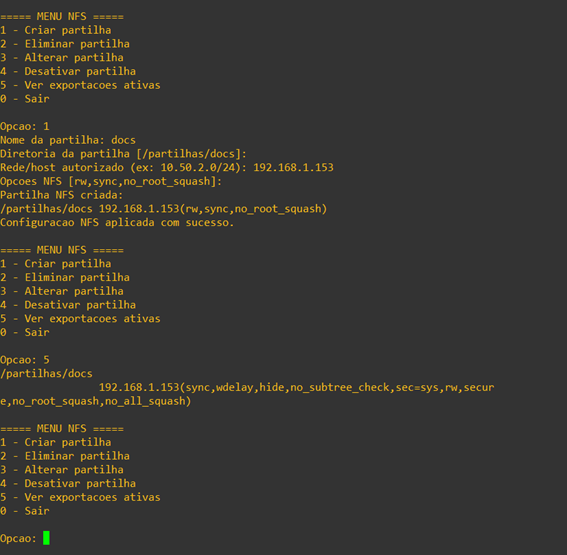
\includegraphics[width=0.78\textwidth,height=0.72\textheight,keepaspectratio]{figuras/q7_menu_criar_listar.png}}{\fbox{\parbox{0.7\textwidth}{Imagem em falta: \texttt{figuras/q7\_menu\_criar\_listar.png}}}}
\caption{Cria\c{c}\~ao da partilha NFS e listagem de exporta\c{c}\~oes ativas}
\end{figure}

\begin{figure}[!htbp]
\centering
\IfFileExists{figuras/q7_exports_verificacao_servidor.png}{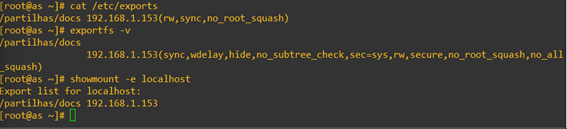
\includegraphics[width=0.78\textwidth,height=0.72\textheight,keepaspectratio]{figuras/q7_exports_verificacao_servidor.png}}{\fbox{\parbox{0.7\textwidth}{Imagem em falta: \texttt{figuras/q7\_exports\_verificacao\_servidor.png}}}}
\caption{Valida\c{c}\~ao no servidor com \texttt{cat /etc/exports}, \texttt{exportfs -v} e \texttt{showmount -e}}
\end{figure}

\begin{figure}[!htbp]
\centering
\IfFileExists{figuras/q7_cliente_mount_df.png}{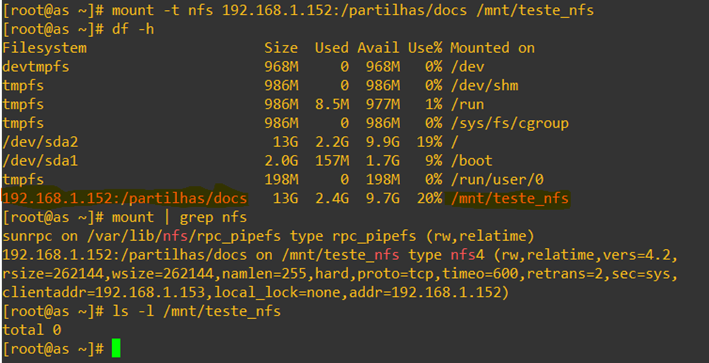
\includegraphics[width=0.78\textwidth,height=0.72\textheight,keepaspectratio]{figuras/q7_cliente_mount_df.png}}{\fbox{\parbox{0.7\textwidth}{Imagem em falta: \texttt{figuras/q7\_cliente\_mount\_df.png}}}}
\caption{Montagem NFS no cliente e verifica\c{c}\~ao com \texttt{df -h} e \texttt{mount | grep nfs}}
\end{figure}

\begin{figure}[!htbp]
\centering
\IfFileExists{figuras/q7_cliente_teste_ficheiro.png}{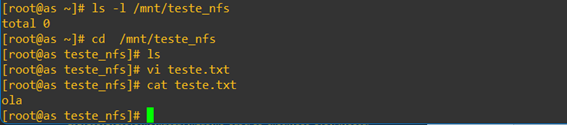
\includegraphics[width=0.78\textwidth,height=0.72\textheight,keepaspectratio]{figuras/q7_cliente_teste_ficheiro.png}}{\fbox{\parbox{0.7\textwidth}{Imagem em falta: \texttt{figuras/q7\_cliente\_teste\_ficheiro.png}}}}
\caption{Cria\c{c}\~ao e leitura de ficheiro no ponto de montagem NFS do cliente}
\end{figure}

\begin{figure}[!htbp]
\centering
\IfFileExists{figuras/q7_servidor_confirma_ficheiro.png}{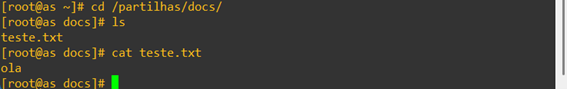
\includegraphics[width=0.78\textwidth,height=0.72\textheight,keepaspectratio]{figuras/q7_servidor_confirma_ficheiro.png}}{\fbox{\parbox{0.7\textwidth}{Imagem em falta: \texttt{figuras/q7\_servidor\_confirma\_ficheiro.png}}}}
\caption{Confirma\c{c}\~ao no servidor do ficheiro criado a partir do cliente}
\end{figure}

\begin{figure}[!htbp]
\centering
\IfFileExists{figuras/q7_menu_alterar_listar.png}{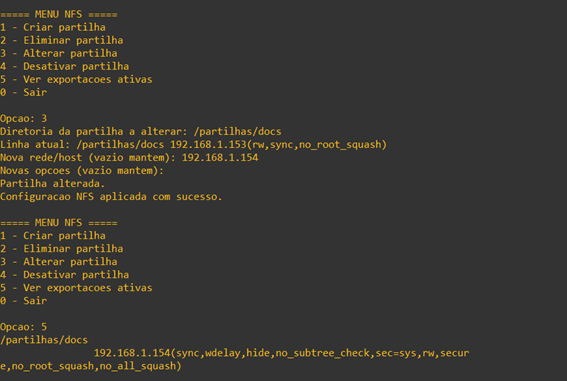
\includegraphics[width=0.78\textwidth,height=0.72\textheight,keepaspectratio]{figuras/q7_menu_alterar_listar.png}}{\fbox{\parbox{0.7\textwidth}{Imagem em falta: \texttt{figuras/q7\_menu\_alterar\_listar.png}}}}
\caption{Altera\c{c}\~ao da rede autorizada e valida\c{c}\~ao da nova exporta\c{c}\~ao}
\end{figure}

\begin{figure}[!htbp]
\centering
\IfFileExists{figuras/q7_menu_desativar_exports.png}{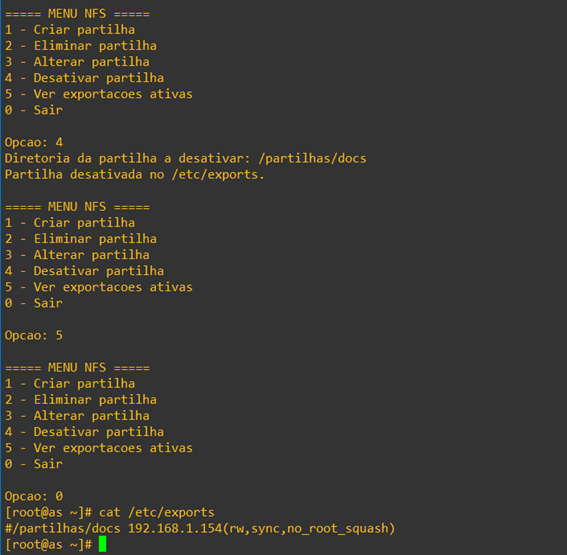
\includegraphics[width=0.78\textwidth,height=0.72\textheight,keepaspectratio]{figuras/q7_menu_desativar_exports.png}}{\fbox{\parbox{0.7\textwidth}{Imagem em falta: \texttt{figuras/q7\_menu\_desativar\_exports.png}}}}
\caption{Desativa\c{c}\~ao da partilha NFS e verifica\c{c}\~ao da linha comentada em \texttt{/etc/exports}}
\end{figure}

\begin{figure}[!htbp]
\centering
\IfFileExists{figuras/q7_menu_eliminar_exports.png}{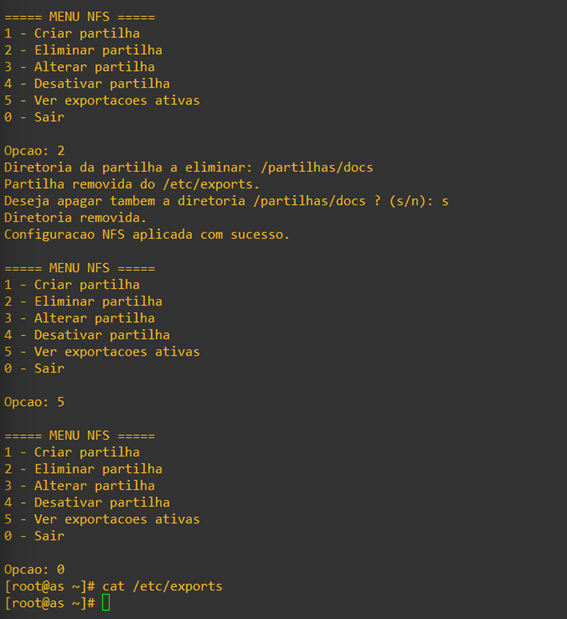
\includegraphics[width=0.78\textwidth,height=0.72\textheight,keepaspectratio]{figuras/q7_menu_eliminar_exports.png}}{\fbox{\parbox{0.7\textwidth}{Imagem em falta: \texttt{figuras/q7\_menu\_eliminar\_exports.png}}}}
\caption{Elimina\c{c}\~ao da partilha NFS e verifica\c{c}\~ao final do \texttt{/etc/exports}}
\end{figure}
